\chapter{Einleitung}
\pagenumbering{arabic}
\section{Aufgabenstellung}
Seit mehreren Jahren bestreitet die \acrshort{hftm} unter der Leitung von Alain Rohr mit dem Solidus Team erfolgreich die internationalen Meisterschaften des RoboCups in der 'Logistics League'.
Das Team kennt sich meisterlich mit der Ansteuerung der Hardware aus, bittet aber die \acrshort{bfh} um Mithilfe beim Software-Engineering.
Die Aufgabe dieser Arbeit ist es, ein Software-Design für die einzelnen Komponenten des verwendeten Roboters zu entwerfen. Angelehnt an die Vorgehensweise 'Domain Driven Design' soll konkret anhand des \acrshort{lidar}s gezeigt werden, wie das erarbeitete Software-Design implementiert und genutzt werden soll. Folgende Merkmale soll das Design mindestens aufweisen:

\begin{itemize}
	\item
	Die Schnittstelle der einzelnen Domänen muss Programmiersprachen-agnostisch sein
	
	\item
	Die Domänen müssen abgekapselt und unabhängig entwickelt und getestet werden können
	
	\item
	Das Design muss klar vorsehen, dass jedes Jahr das Entwicklungsteam komplett ausgetauscht wird
\end{itemize}
Bei dieser Arbeit gilt es auch zu beachten, dass die Software-Fähigkeiten des jeweiligen Entwicklungsteams erst noch ausgebildet werden müssen, es also nötig ist, die Schnittstellen so leicht und verständlich wie möglich zu halten, um nicht eine zu steile Lernkurve als Voraussetzung zu erschaffen.


\bigskip
TODO:
konkrete Aufgabenstellung, was soll raus kommen -> Howto für Studenten der \acrshort{hftm}

\section{HFTM Robocup}
\begin{figure}[htbp]
	\centering
	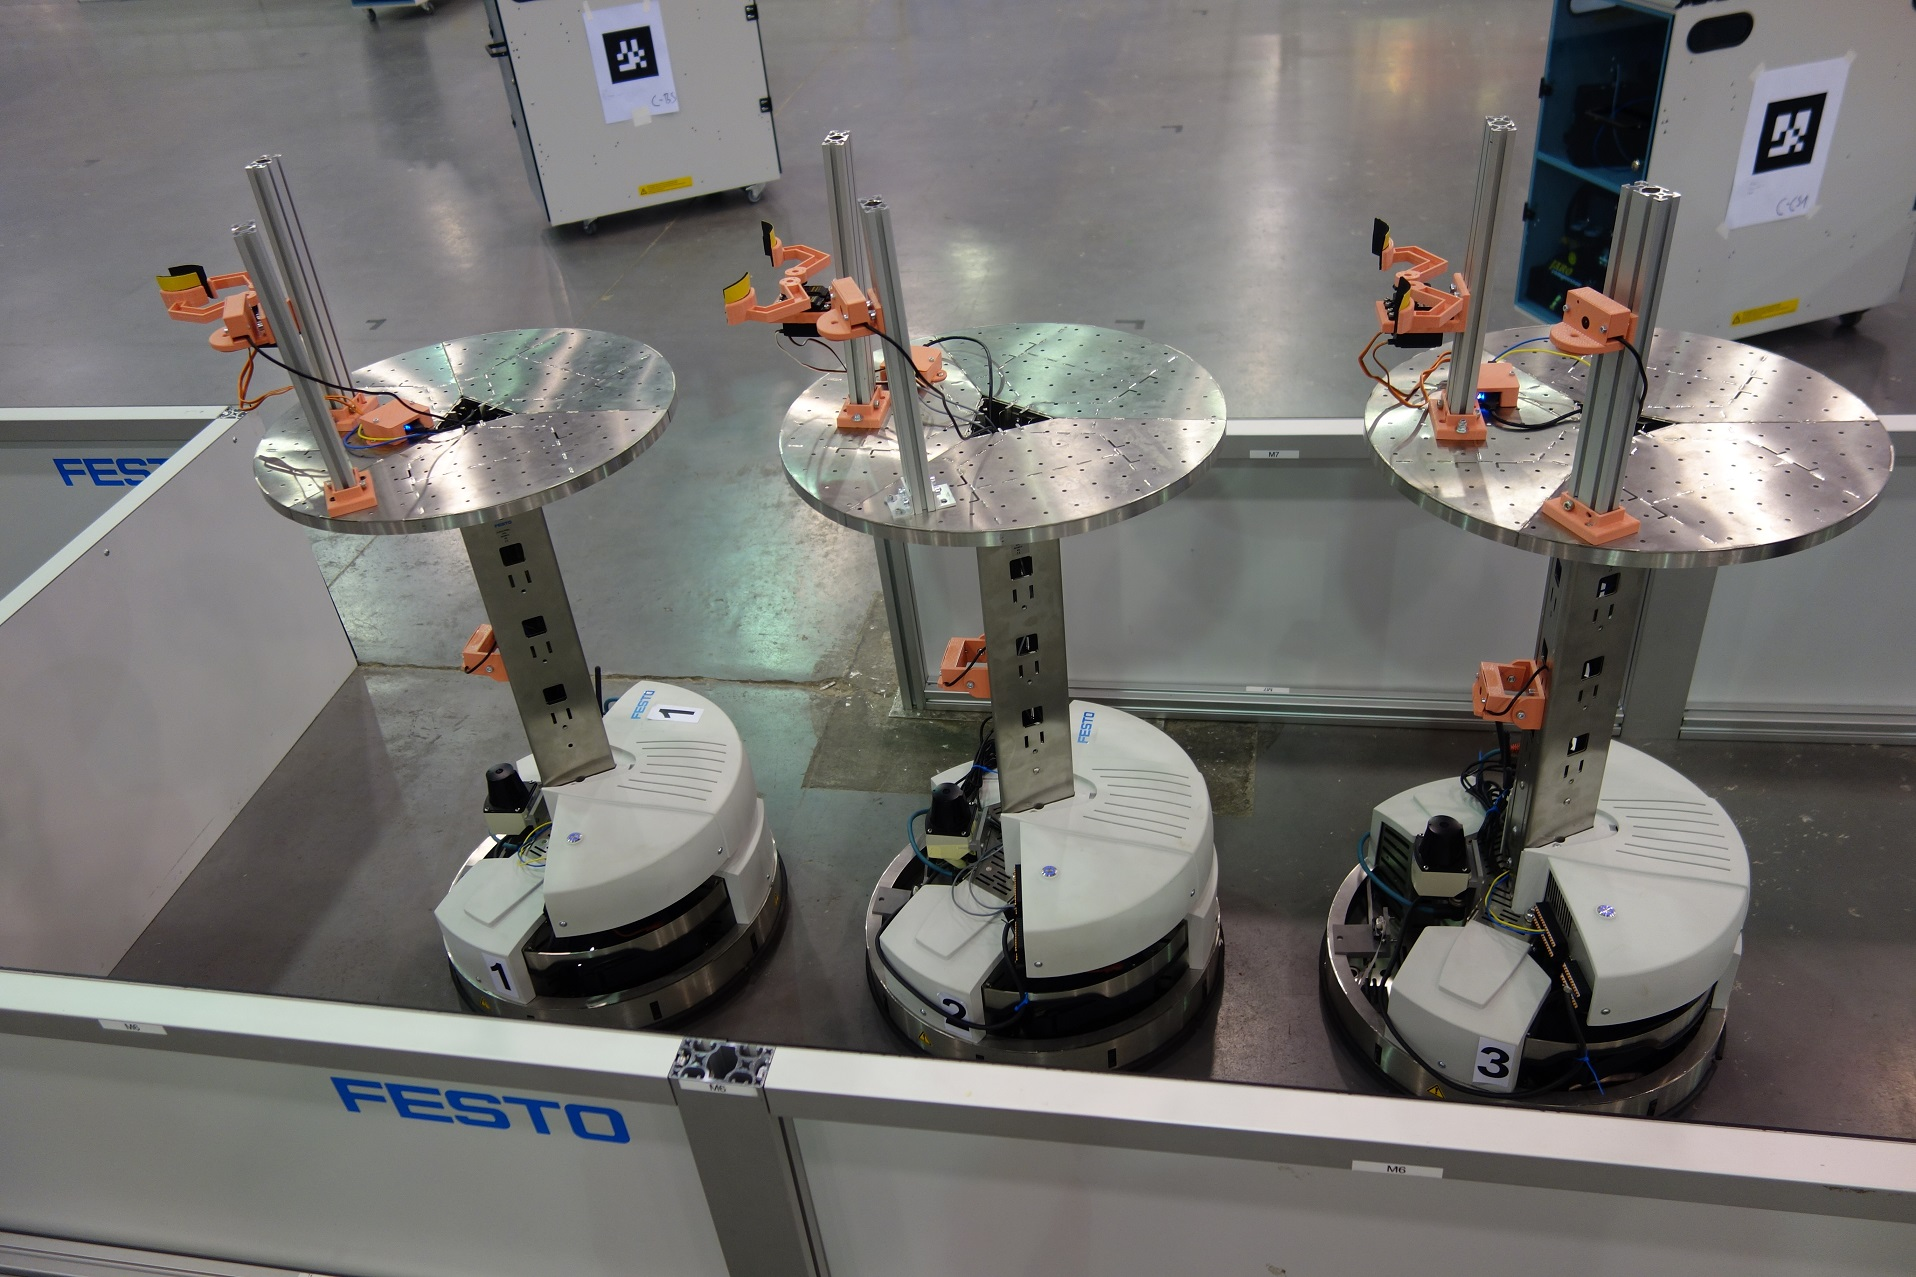
\includegraphics[width=0.5\textwidth]{img/robocup/robotino_v3.jpg}
	\caption{ein Bild\cite{robotino}}  
\end{figure}

TODO:
Roboter erklären, Schule erklären, Studienrichtung?

\section{Lidar}
TODO:
was ist \acrshort{lidar}, wozu wird es verwendet, Funktionsweise High-Level



\section{Vorarbeiten}
Diese Bachelorarbeit basiert nicht auf einer Projekt2-Arbeit. Die ganze Arbeit entsteht also während einem Semester.

\section{Rahmenbedingungen}
Die Rahmenbedingungen dieses Projektes wurden gemeinsam mit dem Betreuer definiert:
\begin{itemize}
\item Source-Code für \acrshort{lidar}-Ansteuerung von \acrshort{hftm}, verwenden als Library
\item Library ch.quantasy.mqtt.gateway\cite{ch.quantasy.mqtt.gateway} von Reto Koenig als Schnittstelle zwischen Hardware, User und Event-Bus
\end{itemize}
